% !TeX root = ../../../master.tex

\subsection{Teilnahme Umfrage}
\label{ssec:UmfrageImplement}

Wie in Abbildung~\vref{fig:UmfrageImplement} dargestellt, soll der Teilnehmer hier auf den zuvor erstellten Fragebogen geleitet werden (vgl. Abschnitt~\vref{ssec:UmfrageErstellen}).
Hier kann dieser diesen ausfüllen und nach Beendigung über einen Knopf abschicken.
% Der Teilnehmer erhält am Ende ein visuelles Feedback, dass seine Teilnahme erfolgreich war.

Abbildung~\vref{fig:UmfrageImplement} stellt eine Umfrage zur Projektmanagement-Vorlesung dar, in der der Teilnehmer drei Fragen beantworten soll.
Exemplarisch sind hierbei drei Fragetypen angeführt:
\begin{itemize}
	\item Multiple Choice: Auswahl der Notationsart für zukünftige Projekte
	\item Skala: Benotung der Vorlesung auf einer Skala von 1 - 5
	\item Ja/Nein: Erneuter Besuch der Vorlesung
\end{itemize}

Über den Knopf \jinline|Complete| kann der Teilnehmer die Umfrage beenden.
Er erhält ein visuelles Feedback über den Status seiner Teilnahme (erfolgreich oder nicht erfolgreich).

\begin{figure}[h]
	\centering
	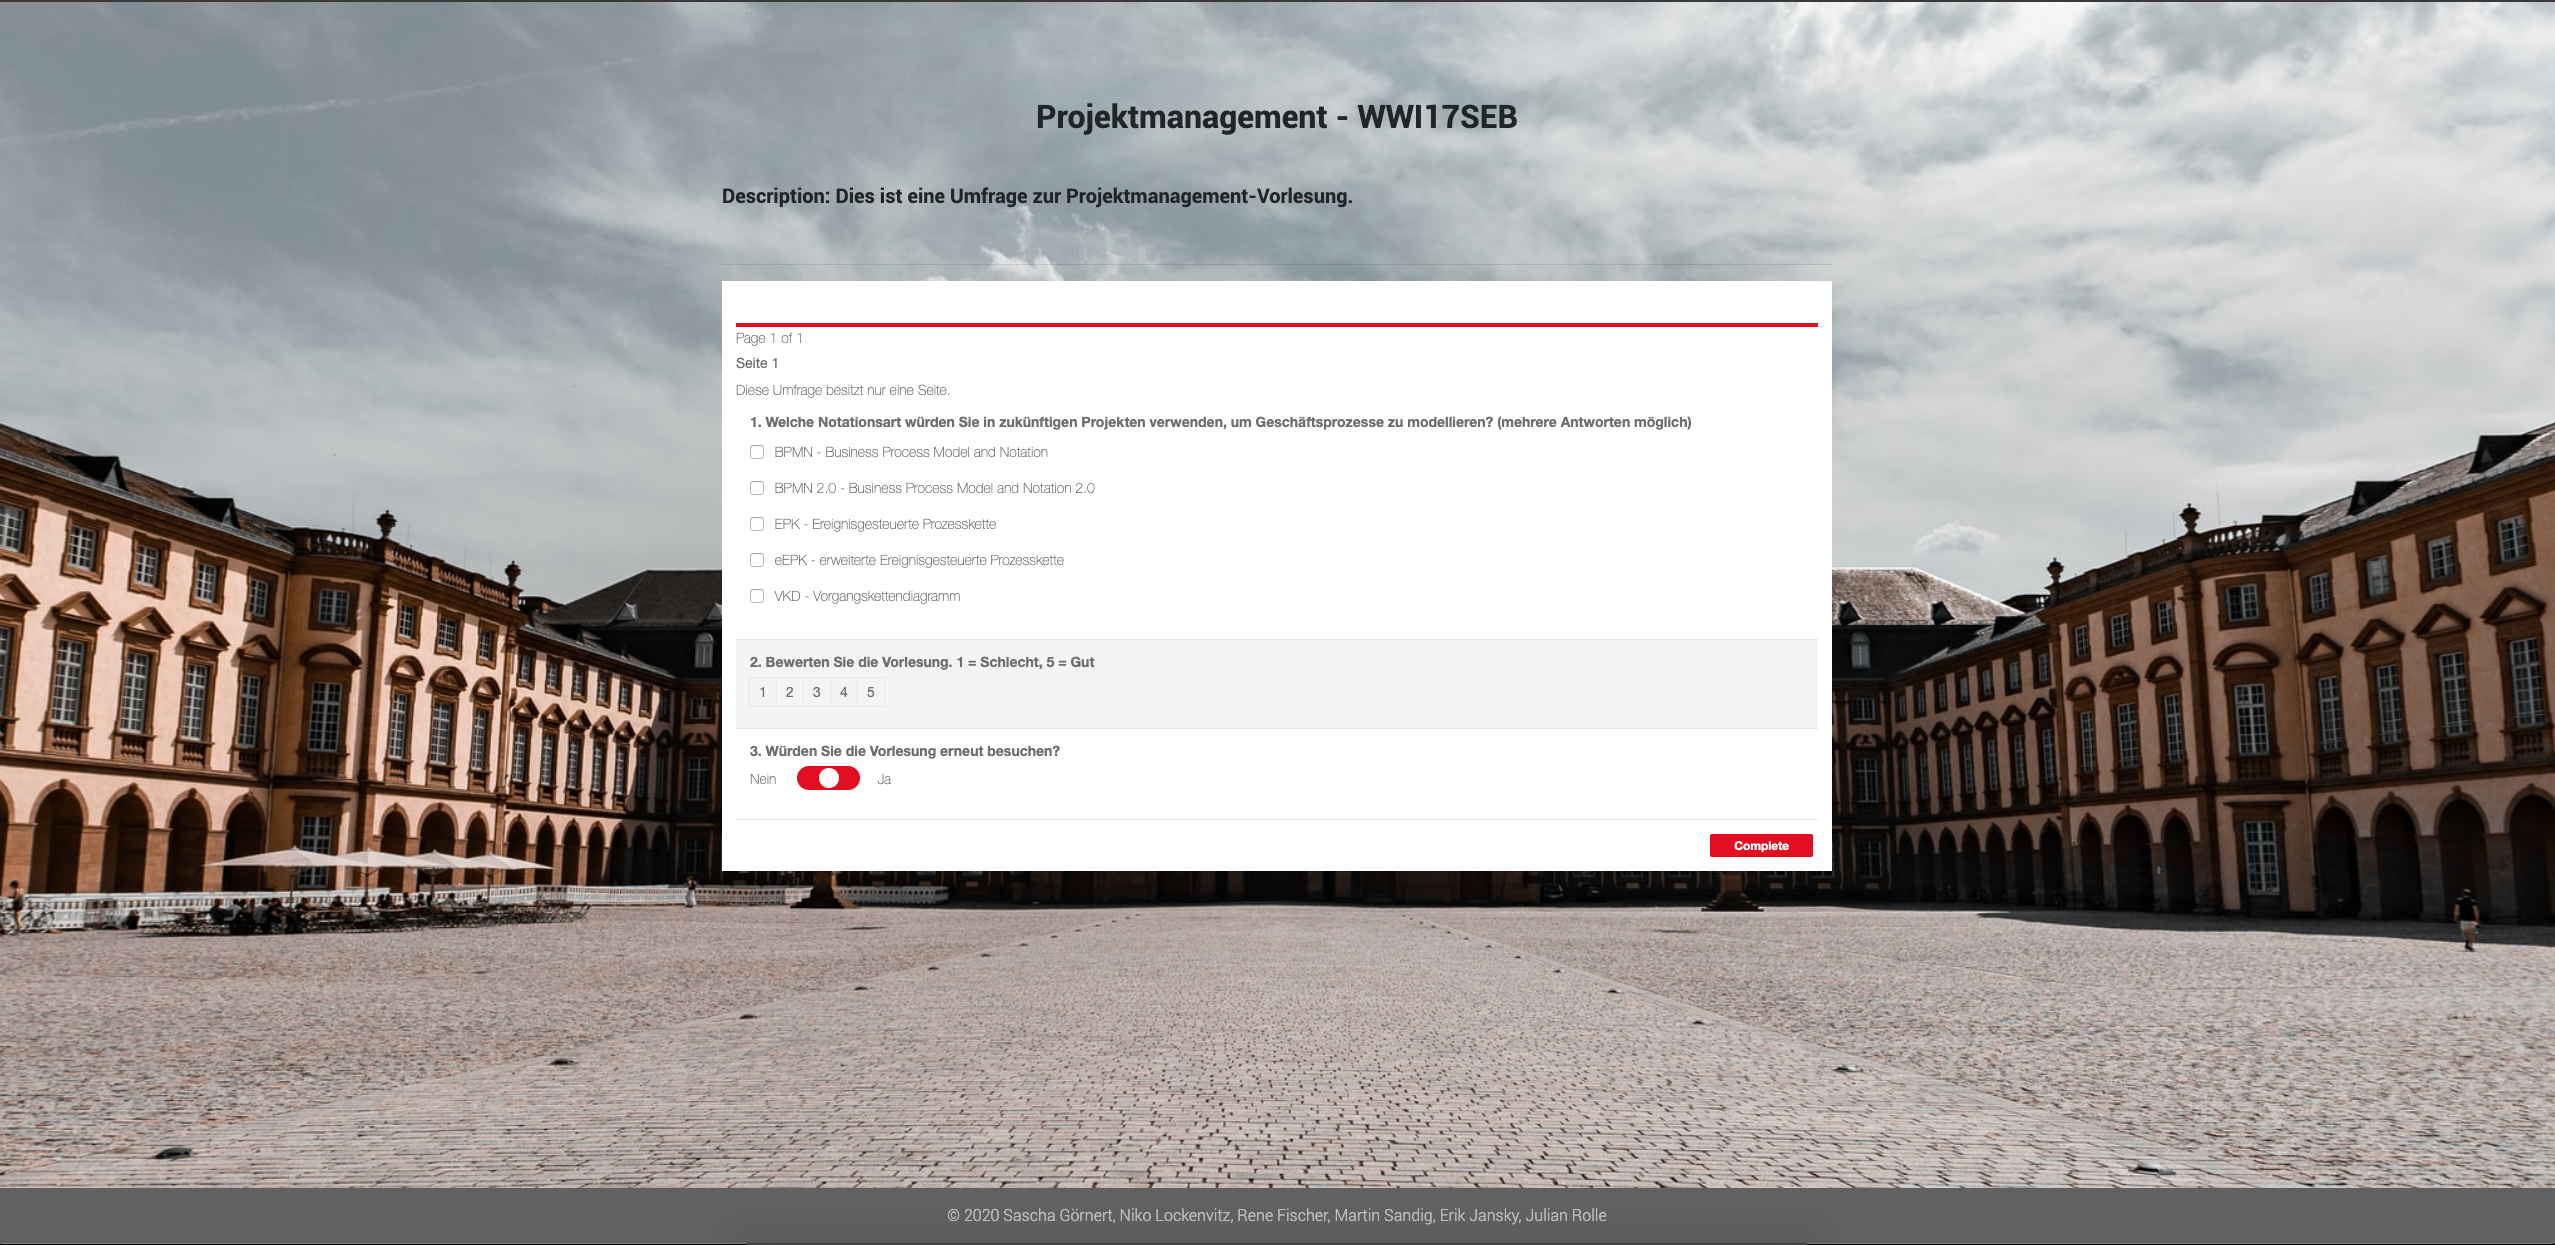
\includegraphics[width=0.95\textwidth, keepaspectratio]{img/client/TeilnahmeUmfrage.png}
	\captionsetup{justification=centering, format=plain}
	\caption[\acl{UI}: Umfrageansicht -- Teilnehmer]{\acl{UI}: Umfrageansicht -- Teilnehmer \\ \quelleScreenshot}
	\label{fig:UmfrageImplement}
\end{figure}
